En este capítulo se justifica la elección y se describe la metodología de desarrollo sobre la que se apoya el proceso de ingeniería. En este proyecto se ha empleado una metodología ágil, Scrum. 



\section{Scrum}

El Scrum es una  Metodología ágil \cite{6} \cite{9} que se usa para estructurar y gestionar proyectos, y para minimizar los riesgos durante la realización del mismo.
Esta metodología esta basada en ciclos iterativos cortos e incrementales, lo que se traduce en una gran flexibilidad a la hora de adaptarse a cambios que surjan duran el desarrollo del proyecto.
Entre las ventajas de Scrum se encuentran la baja carga de burocracia y documentación, productividad, calidad y que se realiza un seguimiento diario de los avances del proyecto, logrando una comunicación activa y constante en el equipo de trabajo.\\
A continuación se describen los principales  de la metodoligía Scrum.


\subsection{Historias de usuario}
Las historias de usuario son los requisitos vistos desde el punto de vista del cliente, es decir, acciones que el usuario llevará a cabo durante el uso del la aplicación. Son las funcionalidades escritas usando frases del lenguaje común del usuario. Son la unidad básica detrabajo y se caracteriza por ser:
\begin{itemize}
\item Independientes.
 \item Negociables.
  \item Estimables.
  \item Pequeñas.
   \item Tangibles.
    
\end{itemize}

Las historias en este proyecto serán las siguientes:


\begin{itemize}
\item Diseño capa intermedia
\item Implementación del servicio Rest
\item Iniciar sesión  
 \item Gestión de puntos de interés (PDI)
  \item Gestión de grupos
  \item Iniciar una ruta individual
   \item Iniciar la ruta compartida
   \item Realización de la memoria.
    
\end{itemize}
 Estas historias anteriormente citadas serán divididas en cada Sprint en pequeñas tareas mas fáciles de manejar. Una tarea es la acción que debe implementar el desarrollador para que se pueda ejecutar parte de la historia, esta está en un lenguaje técnico. Estas tareas reflejan en la mayoría de los casos los denominados casos de uso que comentaremos posteriormente.

\subsection{Sprint}

Por Sprint entendemos un bloque de tiempo fijo, normalmente de 3 o 4 semanas en el que
se crea una versión de nuestra aplicación que se irá incrementando de tamaño
según van avanzando los Sprints. Los Sprints se pueden considerar como pequeños
proyectos ya que al final de cada uno de ellos debemos tener un producto
operativo, es decir, que responda a la historia o historias de usuario planteadas en él.



\subsection{Participantes}
\begin{itemize}
\item \textbf{Product Owner}\\
Es el responsable del producto, de priorizar los user stories y de decidir si el sistema las cumple. En general , es un representante del cliente u otro stakeholder


\item \textbf{Scrum Master}\\
Es el encargado de liderar la reuniones y ayudar al equipo en los problemas que tengan  en la implementación de la metodología. Debe minimizar las imposibilidades que surgen en el desarrollo del proyecto para que se cumplan los objetivos. Además debe promover la comunicación entre los integrantes del grupo para generar la motivación necesaria para conseguir los objetivos en plazo.




\item  \textbf{Scrum Team}\\
Son los encargados de desarrollar y llevar acabo las tareas de los sprints. En si son quienes realizan las tareas que finalmente generan el producto que se va a entregar.


\item  \textbf{Cliente}\\
Recibe el producto y puede influir en el proceso, entregando sus ideas o comentarios respecto al desarrollo a través del feedback con el product owner y el equipo sobre las versiones del producto. 
\end{itemize}

\subsection{Cómo funciona el Proceso}



\begin{figure}
		\centering
		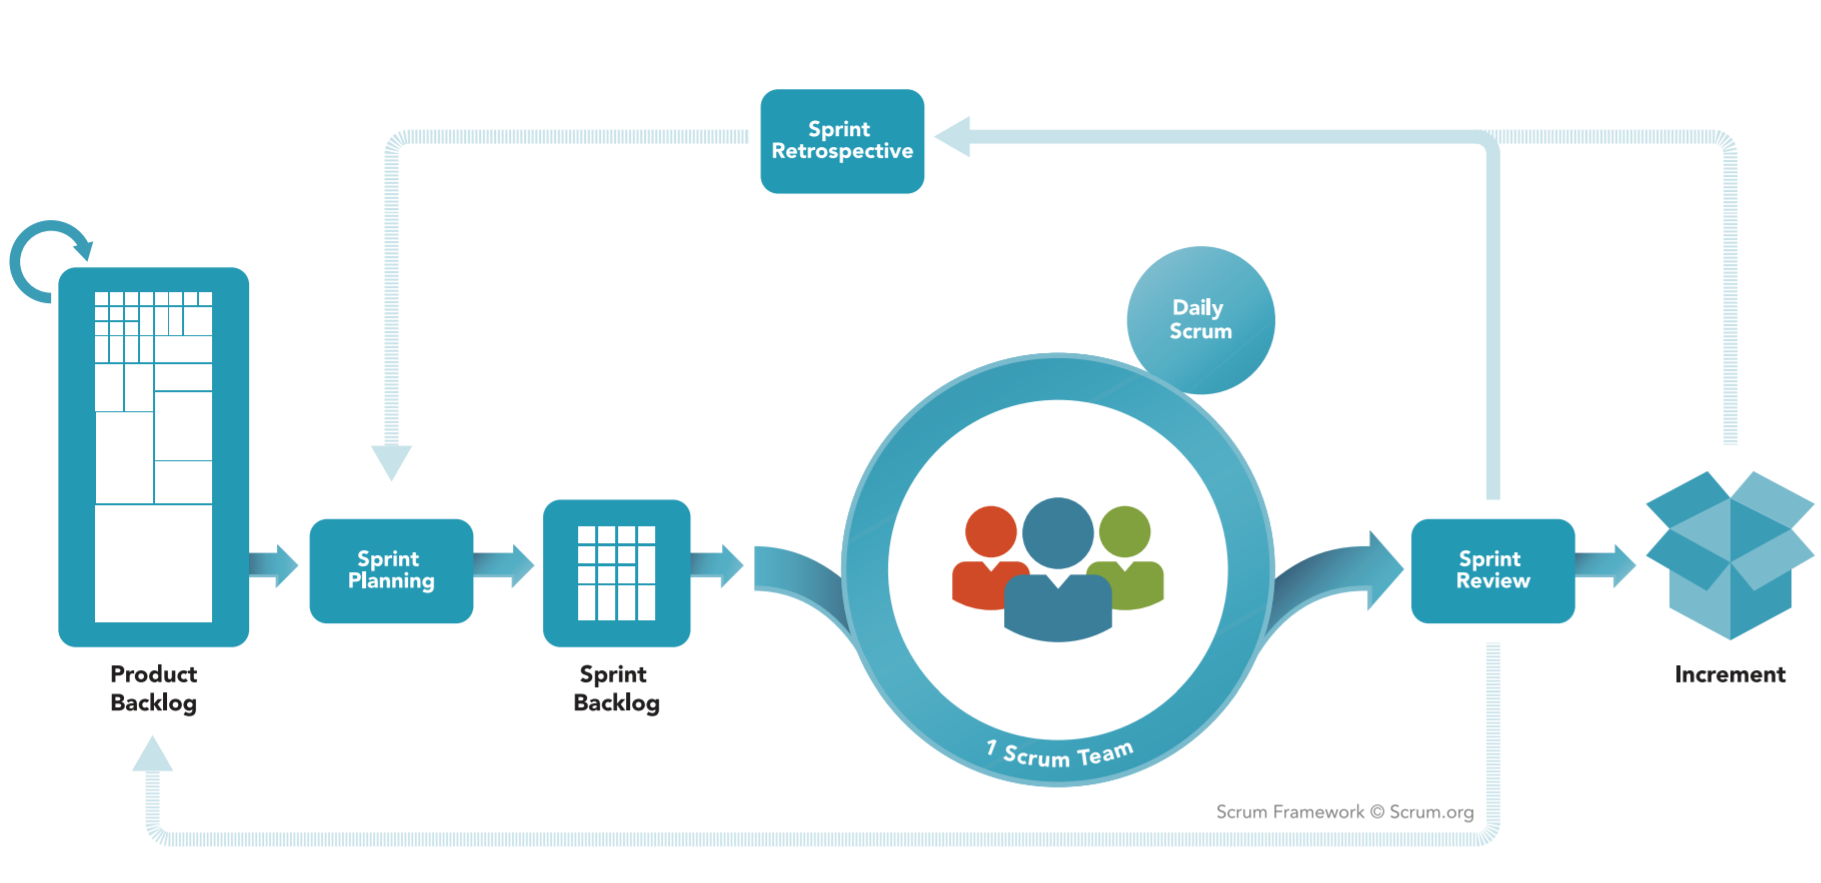
\includegraphics[width=\textwidth] {scrum.jpg}
		\caption{Metodología Scrum }
		\label{fig:scrum}
	\end{figure} 


El proceso general se puede ver en la figura~\ref{fig:scrum}. El proceso comienza con la definición del Product Backlog. De este Product Backlog  se irán obteniendo las historias para los distintos sprints. . A continuacion comentaremos sus partes:
\begin{itemize}
\item \textbf{Definición del Product Backlog}. 
Es una lista con las funcionalidades de la aplicación.
Estas funcionalidades que se definen en el Product Owner son las historias del usuario, es decir, es lo que el usuario quiere hacer en la aplicación y por tanto en muchos casos cada historia puede contener varios casos de uso. \\
Está elaborado por el Product Owner y las funcionalidad están ordenadas de mayor a menor importancia para el cliente. La finalidad del Product Owner es plantear lo que hay que hacer.
Con las historias ordenadas se indicarán los Sprints que serán necesarios pudiendo hacer  varias historias en un mismo Sprint pero nunca una historia dividida en dos Sprints. 

 



\item \textbf{Sprint Planning Meeting}. Figura~\ref{fig:planing}\\
 Esta reunión se hace al comienzo de cada Sprint y se define cómo se va a enfocar el sprint, se revisan las historias con mayor prioridad y se decide el Sprint backlog.
\begin{figure}[H]
		\centering
		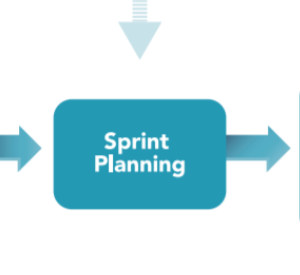
\includegraphics[width=0.3\textwidth] {planing.png}
		\caption{Parte metodología Scrum, Sprint Planning }\label{fig:planing}
	\end{figure} 

\item \textbf{Sprint Backlog}. 
Es el conjunto de historias del Product Backlog que se decidirán hacer en el Sprint, estando ordenadas de mayor a menor prioridad. 

\begin{figure}[H]
		\centering
		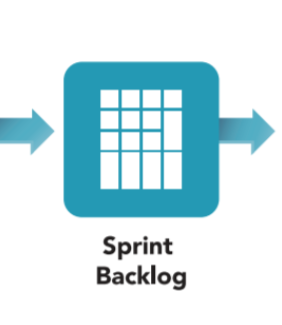
\includegraphics[width=0.3\textwidth] {sprint.png}
		\caption{Parte metodología Scrum, Sprint Backlog }\label{fig:sprint}
	\end{figure} 

 
 
\item \textbf{Daily Scrum o Stand-up Meeting. Figura~\ref{fig:daily}}\\
Es una reunión breve que se realiza cada mañana mientras dura el periodo de Sprint. 
En estas reuniones si algún miembro del equipo encuentra algún problema  se comenta y se trata de buscar la solución. El scrum master es el encargado de gestionar la resolución de los inconvenientes encontrados.

\begin{figure}[H]
		\centering
		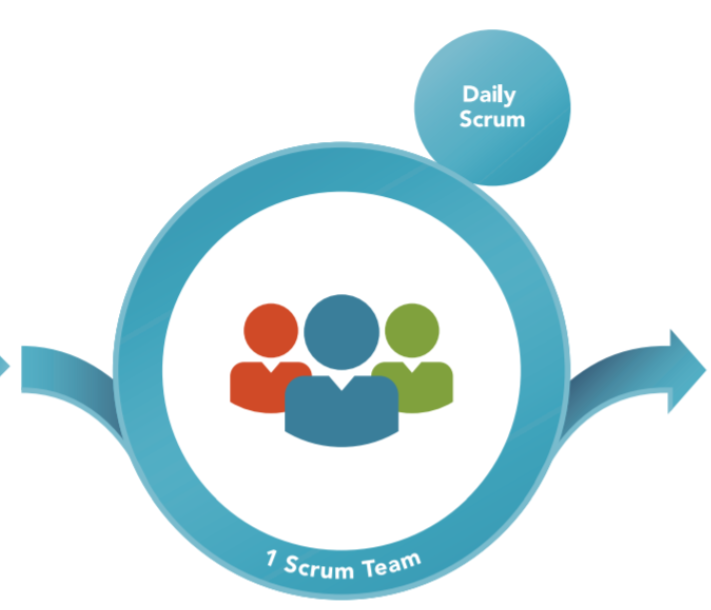
\includegraphics[width=0.3\textwidth] {daily.png}
		\caption{Parte metodología Scrum, Daily Scrum }\label{fig:daily}
	\end{figure} 

\item\textbf{ Sprint Review}\\
Esta sería la primera reunión una vez acabado el Sprint. En ella se deberían revisar las tareas acabadas y se debería ver un avance claro para ser presentado al product owner y al cliente. Las tareas inacabas las deberían ser devueltas al Product Backlog y si hiciera falta volver a calcular las prioridades.

 \item \textbf{Sprint Retrospective}\\
  El equipo revisa los objetivos cumplidos del Sprint terminado. Se anota lo bueno y lo malo, para no volver a repetir los errores. Esta etapa se centra en el cómo se realiza el proyecto para ver si hay algún error en el desarrollo poder resolverlo en el siguiente Sprint.
\end{itemize}



\section{Adaptación la metodología a este proyecto }
 Debido a la naturaleza de un Trabajo de fin de grado  debimos realizar una serie de cambios o adaptaciones en ciertos elementos como fueron los siguientes:
\subsection{Participantes}
Los participantes fueron los siguientes:
\begin{itemize}
\item El Product Owner interpretado por los  directores y por el alumno.
\item El rol  cliente también fue desempeñado por los directores.
\item El Scrum Master no se usó puesto que se decidió 
 user scrum program.
\item  Y el equipo solo estuvo formado por el alumno.

\end{itemize}

\subsection{Sprints}
Cada sprint siempre tuvo una duración establecida de 4 semanas y 5 horas cada día aunque la carga de trabajo variaba en algún Sprint.
En el capítulo \ref{ejec} de detallan los sprints en que se estructuró el proyecto, los objetivos y duración de cada uno de ellos.

\subsection{Reuniones}

En el apartado de las reuniones al iniciar y al finalizar cada Sprint se realizaban reuniones con los directores y se aprovechaba para la planificación de la siguiente. Como también durante ellos para resolver dudas.\\

Una vez adaptada la metodología a este proyecto encontramos las siguientes ventajas a su uso:

\begin{itemize}
\item Ayuda a estar más centrado en el producto durante el desarrollo del proyecto ya que no existe la preocupación por establecer las siguientes tareas.  Estas ya quedaron indicadas en el sprint. 



\item En ocasiones al ir avanzando en el desarrollo aparecen nuevas funcionalidades que se pueden ir añadiendo al Product Backlog. Esto lo podemos hacer siempre y cuando nos ciñamos al Sprint Backlog
 para saber la tarea que realizar en ese momento.


\item  Las historias de usuario se van dividiendo en tareas que se puedan realizar durante el sprint. De este modo una vez acabado el sprint tenemos un producto potencialmente entregable.\\

Dado el poco conocimiento de la metodología Scrum antes de la realización del proyecto, el ir avanzando en el proceso ayuda a adquirir conocimientos, los cuales ayudarán a estimar mejor la duración e importancia de los elementos que se añaden al Sprint Backlog.


\item
Durante el desarrollo del proyecto hay ciertas funcionalidades que pueden cambiar. Empleando los principios de las metodologías ágiles en cada iteración haremos que el proyecto sea mas adaptable antes nuevos requisitos y cambios.

\end{itemize}
